% Reliability-Aware Hybrid Retrieval for Natural-Language-to-Shell-Command Assistance
% ACL/EACL Student Research Workshop, long paper -- FINAL / CAMERA-READY VERSION.
%
% This is a thin wrapper: the actual paper body lives in content.tex, shared identically with
% main_review.tex (the anonymized double-blind version). Edit content.tex for any content change
% -- editing only one of the two wrappers would silently desync the submission versions.
%
% Author identity IS shown in this version (no anonymization, no line numbers). If this needs to
% go into double-blind review, use main_review.tex instead, not this file.

\documentclass[11pt]{article}
\usepackage{acl}
\usepackage{times}
\usepackage{latexsym}
\usepackage[T1]{fontenc}
\usepackage[utf8]{inputenc}
\usepackage{microtype}
\usepackage{graphicx}
\usepackage{booktabs}
\usepackage{amsmath}
\usepackage{amssymb}

\title{Reliability-Aware Hybrid Retrieval for Natural-Language-to-Shell-Command Assistance: \\ A Non-LLM Study}

\author{
  Manoj Kumar Gaddam \\
  SRKR Engineering College \\
  \texttt{manojgaddam133@gmail.com}
}

\begin{document}
\maketitle

% Shared paper body, included identically by both main.tex (final/camera-ready) and
% main_review.tex (anonymized review mode). Edit ONLY this file for content changes -- editing the
% body in one wrapper and not the other would silently desync the two submission versions.

\begin{abstract}
Natural-language interfaces to the shell are usually framed as generation (NL2Bash, NL2SH). We study a
constrained alternative --- closed-vocabulary \emph{retrieval} from a curated command library, with no large
language model anywhere in the system --- and focus on \emph{reliability} rather than accuracy alone. A real,
previously shipped BM25 baseline reaches 67.3\% accuracy on a 150-query benchmark but has 86.06\% mean
confidence on its wrong answers. We test whether a lightweight hybrid lexical+local-semantic retriever with
post-hoc isotonic calibration and margin-based rejection improves accuracy and reliability, under leakage-free
nested 5-fold cross-validation, on two benchmark versions: v0.1 (150 queries) and v0.2, which adds 35
out-of-domain (OOD) and 24 ambiguous queries to v0.1, so the two are not independent samples. Calibration is the
most robust result: it reduces the expected calibration error (ECE) of the hybrid's confidence by 80\% (v0.1) and
77\% (v0.2), is the only one of four compared effects significant after Holm--Bonferroni correction on both
versions (adjusted $p=0.0004$ and $0.0003$), and persists on intents held out from tuning (76\% and 69\%) and when
ambiguous queries are removed. OOD rejection, underpowered at 15 queries (raw $p=0.25$), is significant on v0.2's
50 OOD queries (34\%$\to$68\%; adjusted $p=0.00006$). The hybrid's accuracy gain over BM25 is consistent in size
(+5.2 and +3.8 points) but statistically fragile (adjusted $p=0.047$ on v0.1; raw $p=0.070$ on v0.2, where BM25
wins on exactly one query), and its advantage over dense retrieval on v0.2 (adjusted $p=0.025$) is no longer
significant without bare-keyword ambiguous queries (raw $p=0.057$). Ambiguity detection is weak (F1 0.31--0.50).
A rule-based safety classifier reaches 95\%/95\% precision/recall in flagging risky commands. A blind
re-annotation of 14 of v0.2's 59 AI-authored queries by one partially independent reviewer gave Cohen's
$\kappa=0.63$, below our 0.7 target; all 8 sampled OOD labels were confirmed, and every disagreement concerned an
ambiguous label. All significance analyses were specified after the raw results were seen and are exploratory.
\end{abstract}

\section{Introduction}

Natural-language shell assistance can lower the barrier to command-line tools, but incorrect
commands --- especially destructive ones --- carry real cost. The dominant research trajectory
since NL2Bash \citep{lin-etal-2018-nl2bash} has been generative: seq2seq and Transformer models (the
NLC2CMD competition, \citealp{agarwal2021nlc2cmd}), then LLM-based systems (NL2SH;
\citealp{westenfelder2025nl2sh}), most recently with execution-grounded, RL-trained approaches
(BashCoder-R1; \citealp{yu2026bashcoderr1}). This trajectory inherits a persistent risk:
open-vocabulary generation can hallucinate syntactically valid but semantically wrong or unsafe
commands.

We study a different, narrower approach implemented in a real, previously-shipped, in-use npm
package: retrieval from a fixed, curated command corpus (279 commands on the evaluated Windows
platform) using classical lexical (BM25) scoring, with no LLM anywhere in the system. This constrains
coverage but structurally eliminates hallucination of arbitrary commands. We audited and reproduced the
system's baseline behavior (\S\ref{sec:system}) and found a specific, serious problem: the system is
frequently \emph{confidently} wrong, not merely wrong. This paper asks whether that problem, and the
system's accuracy more broadly, can be improved without abandoning the no-LLM, fully-offline design
constraint.

Given a natural-language query and a fixed corpus of \texttt{(intent, command, category,
description, os)} tuples, the task is to return the single best-matching command, or explicitly
decline to answer if no corpus entry is a confident match --- retrieval, not generation, over a
closed output space, unlike NL2Bash-style tasks where the model may emit any syntactically valid
command string.

\paragraph{Research question.} Can a lightweight hybrid lexical+local-semantic retrieval
architecture, combined with explicit uncertainty estimation and post-hoc calibration, measurably
improve accuracy and reliability over a pure-BM25 baseline, without the cost or hallucination risk
of a generative system?

\paragraph{Contributions.} (1) A reproduced audit of a real shipped BM25 baseline's accuracy and ---
more consequentially --- its confidence miscalibration. (2) A five-component reliability-aware
retrieval architecture evaluated under leakage-free nested cross-validation. (3) Results on two
benchmark versions (v0.2 extends v0.1, so they are not independent), with Holm--Bonferroni-corrected
significance and a sensitivity analysis showing which conclusions depend on bare-keyword ambiguous
queries. (4) An intent-held-out (GroupKFold) generalization check. (5) Disclosure of the null, weak,
and fragile results we found, including a below-target blind re-annotation of a sample of our own
benchmark's AI-authored queries.

\section{Related Work}

NL2Bash \citep{lin-etal-2018-nl2bash} introduced a corpus of English descriptions paired with Bash
commands, with neural baselines and the BLEU and template-match evaluation this field has used
since. The NLC2CMD competition \citep{agarwal2021nlc2cmd} introduced a utility+flag-overlap metric more
tolerant of near-miss answers than exact match. NL2SH \citep{westenfelder2025nl2sh} is a recent
generation-based successor, reporting that parsing, in-context learning, in-weight learning, and
constrained decoding improve LLM translation accuracy by up to 32\%. Recent work reinforces our framing
that exact-match accuracy alone is an incomplete signal: QuoteBench \citep{li2026quotebench} shows that
matched execution scores can mask command-path failures, and BashCoder-R1 \citep{yu2026bashcoderr1},
despite RL training against execution feedback, reaches 90\% (single-line) and 73\% (multi-line) full
functional success. A 2026 scaling study \citep{wang2026bm25wins} finds BM25 overtakes dense and agentic
retrieval past roughly 10M corpus tokens, supporting lexical retrieval's competitiveness at scale, though
at a corpus scale far larger than ours. \citet{notaro2024commandrisk} train a transformer-based
command-risk classifier; we deliberately compare against a simpler, fully deterministic rule-based
alternative (\S\ref{sec:ablation}). Our study complements this generation-focused work with a
reliability-oriented evaluation of closed-vocabulary retrieval: calibration, OOD rejection, and
intent-held-out evaluation of a lexical/hybrid retriever. We do not claim priority; our literature search
was limited (see Limitations).

\section{TermAssist: Baseline System and Benchmark}
\label{sec:system}

\paragraph{Baseline architecture} (frozen for this study): tokenize (lowercase, strip punctuation,
10-word stopword list), BM25 scoring ($k_1=1.2$, $b=0.75$, standard IDF smoothing) over
\texttt{intent+category+description}, plus a flat $+15.0$ bonus when the query is a near-substring
of the command's intent. Confidence $= \min(\mathrm{round}(\mathrm{score}/8\times100), 100)$,
rejected below $\mathrm{score}<2.0$. No embeddings, no LLM, mean latency 3.29ms. We reproduced this
baseline's outputs exactly (0/150 mismatches against the archived results).

\paragraph{Corpus.} 431 records in 27 categories, covering 297 distinct intents across platforms; each
record is tagged for Windows, Linux/macOS, or all platforms. On the evaluated Windows platform the 152
Linux/macOS-only records are filtered out, so the system searches \textbf{279 records (145 cross-platform,
134 Windows-specific), each a distinct intent}; this is the corpus size we use throughout. The records are
curated but were checked by script rather than validated one by one, and a few Windows-visible records are
Linux commands (e.g., \texttt{sudo reboot}). A planned expansion to 500--800 human-validated intents is not
complete, so all results here are on this 279-intent corpus.

\paragraph{Benchmark, v0.1.} 150 hand-adjudicated queries across 9 types (canonical, paraphrase,
low-overlap-paraphrase, ambiguous, OOD, polysemy, single-keyword, safety-sensitive,
complex-multi-intent), with ground-truth classification (119 CORRECT, 14 AMBIGUOUS, 15 OOD, 2
NEEDS\_CORRECTION) and a risk-level field (120 LOW, 10 MEDIUM, 15 HIGH, 5 CRITICAL) reused in the
safety evaluation (\S\ref{sec:ablation}).

\paragraph{Benchmark, v0.2.} A second version (209 queries) \emph{extends} v0.1: it contains all 150
v0.1 queries plus 35 new OOD and 24 new ambiguous queries, added because v0.1's OOD (15) and ambiguous
(14) subsets were too small for adequately powered tests. It is therefore an expanded benchmark, not an
independent sample: the 121 answerable queries are identical in both versions, and every difference
between the versions comes from the added OOD and ambiguous queries. The new queries were authored and
adjudicated by an AI agent under human direction, following v0.1's design methodology (each query
checked against actual system retrieval output; 6 of 30 drafted ambiguous candidates were rejected for
failing the ambiguity or novelty criteria). Seventeen of the 24 new ambiguous queries are single-token
tool or category names (``grep'', ``pip'', ``system''); we call these \emph{bare-keyword} queries, and
nine of v0.1's 14 ambiguous queries are of the same kind (``git'', ``docker'').

\paragraph{Ground-truth defects.} Three items have ground truth outside the corpus the system searches:
\mbox{TA-B187} (``tar''), whose gold and acceptable commands exist only among the Linux/macOS records;
\mbox{TA-B145}, whose gold command is not in the corpus (it is already labeled NEEDS\_CORRECTION); and
\mbox{TA-B149}, one of whose acceptable commands is not in the corpus. Every system misses \mbox{TA-B145} and
\mbox{TA-B187} and answers \mbox{TA-B149}
correctly, so no comparison between systems changes, but the two unanswerable items understate every
system's non-OOD accuracy by up to 0.7 points on v0.1 (1/135) and 1.3 points on v0.2 (2/159). We report
both versions unchanged.

\paragraph{Baseline results (v0.1).} Overall accuracy 67.3\% (101/150); supported-task (non-OOD)
accuracy 71.9\%; OOD rejection 26.7\% (73.3\% false-acceptance); success on the 14 AMBIGUOUS-labeled
queries 28.6\%. By query type (a finer grouping than the labels): canonical/safety-sensitive 100\%,
paraphrase 88.0\%, complex-multi-intent 86.7\%, polysemy 55.6\%, ambiguous 58.3\%,
low-overlap-paraphrase 33.3\%, OOD 26.7\%, single-keyword 0.0\%. Mean confidence on the 49 wrong
(non-rejected) predictions: \textbf{86.06\%}, with 44.9\% of failures at exactly 100\% confidence ---
the central problem motivating this paper.

\section{Reliability-Aware Retrieval Architecture}
\label{sec:architecture}

Five components, each targeting a specific measured failure: (1) local dense retrieval
(\texttt{Xenova/all-MiniLM-L6-v2}, 384-dim, offline after one-time download) for the lexical gap;
(2) hybrid score fusion with $\alpha$ tuned via nested 5-fold CV; (3) margin/entropy uncertainty
signals over top-10 ranked candidates; (4) OOD and ambiguity detectors (dev-tuned thresholds); (5)
isotonic confidence calibration. A sixth, independent component --- a rule-based safety classifier
--- targets command risk, orthogonal to retrieval correctness. No LLM is used anywhere in the
system. Dense-only retrieval took 5.9\,ms per query on average on v0.1 (BM25: 3.3\,ms) once the model
was loaded; we did not time the full hybrid pipeline end to end.

\section{Experimental Methodology}
\label{sec:methods}

All tuned parameters (fusion $\alpha$, OOD/ambiguity thresholds) are selected via nested 5-fold
cross-validation (seed 42, stratified by classification) --- \textbf{Split A}: for each test fold,
the parameter is chosen using only the other four folds, then applied once to the held-out fold,
never tuned on data it is later scored against. Accuracy is pooled over all non-OOD queries (hits
divided by queries), the unit of our significance tests; per-fold means differ from it by at most
0.2 points. Statistical testing uses the exact (binomial) McNemar's test, given small discordant-pair
counts.

\paragraph{Multiple-comparison correction.} We fix a family of four comparisons per benchmark
version --- accuracy vs. BM25, accuracy vs. dense-alone, OOD rejection, and calibration ECE
reduction --- and apply Holm--Bonferroni correction within each family; a result is called significant
only at Holm-adjusted $p<0.05$. \emph{This family was written down after the raw v0.1 and v0.2 test
results had been computed} (only the Holm-adjusted values and bootstrap intervals came later), and
calibration was named the primary hypothesis knowing it was the robust result. All significance
statements here are therefore exploratory with respect to these data; the specification would be
confirmatory only on a benchmark built after it. The two families are also not independent, since
v0.2 contains v0.1.

\paragraph{Bootstrap confidence intervals.} Percentile bootstrap (10,000 resamples, seed 42)
provides 95\% CIs for the accuracy deltas (paired resampling over non-OOD query ids) and for the
calibration ECE reduction (resampling over pooled held-out predictions), complementing the discrete
exact McNemar's test with a continuous-estimate view of the same comparisons.

\paragraph{Split B --- intent-held-out generalization.} To test whether Split A's findings depend on
the same command intents appearing in both tuning and test folds, we additionally construct a
GroupKFold split keyed by a derived intent-group id (the gold command for answerable queries; the
sorted acceptable-command set for ambiguous queries; a singleton per query for OOD queries, which
target no intent). We run this on both benchmark versions (171 groups over v0.2's 209 queries; 125
groups over v0.1's 150 queries), both verified programmatically to place zero groups across more
than one fold, so $\alpha$, the detector thresholds, and the isotonic calibrator are always selected
on queries targeting \emph{different} command intents than those they are scored on.

\section{Results}
\label{sec:results}

\paragraph{Retrieval accuracy.} On v0.1's 135 non-OOD queries, BM25 reaches 71.9\% (97/135), dense-only
72.6\% (98/135), and hybrid 77.0\% (104/135): a gain over BM25 of $+5.2$ points (bootstrap 95\% CI [2.2,
8.9]; exact McNemar $p=0.0156$, Holm-adjusted $p=0.047$: significant, but by 0.003). On v0.2's 159 non-OOD
queries, BM25 reaches 75.5\% (120/159), dense-only 72.3\% (115/159), and hybrid 79.2\% (126/159): a gain of
similar size ($+3.8$ points, CI [0.6, 7.5]) that does not clear $p<0.05$ even before correction (raw
$p=0.070$). The exact test rests on very few discordant queries: 7 on v0.1 (all favoring hybrid) and 8 on
v0.2 (7 favoring hybrid). The single query on which BM25 succeeds and hybrid fails is the bare keyword
``system'' (\texttt{TA-B194}); without it the v0.2 comparison is 7--0, exactly as on v0.1. The accuracy gain
is therefore consistent in size across versions, but its significance depends on one query, and we read it
as suggestive rather than established. Hybrid vs.\ dense-alone is not significant on v0.1 (Holm-adjusted
$p=0.292$) but is on v0.2 (Holm-adjusted $p=0.025$); three of the 14 queries on which hybrid beats dense are
new bare-keyword queries (\texttt{jq}, \texttt{grep}, \texttt{shell}), and without them the comparison is
3--11 (raw $p=0.057$). We suspect exact-token matching helps on such queries, but we did not test this.

\begin{figure*}[t]
  \centering
  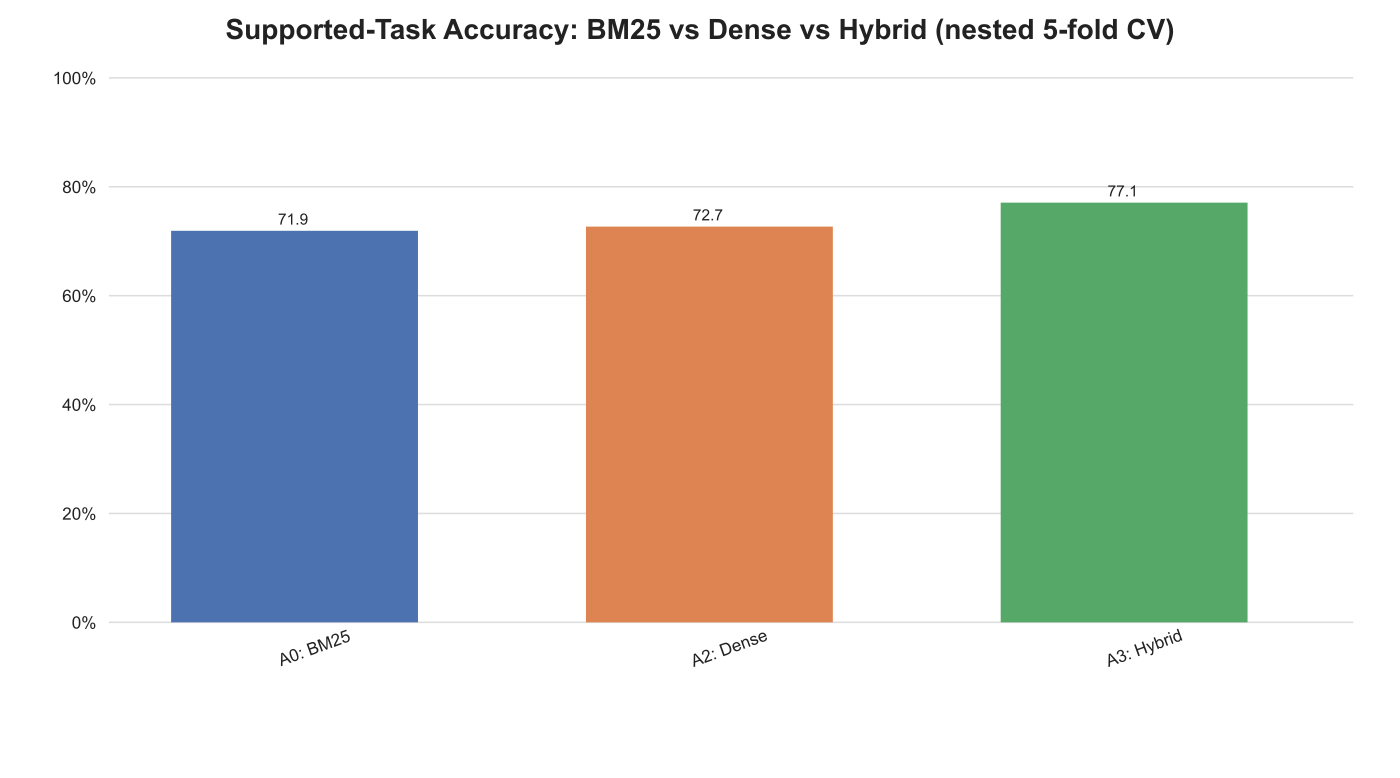
\includegraphics[width=0.48\linewidth]{figures/fig1_baseline_vs_improved_accuracy.png} \hfill
  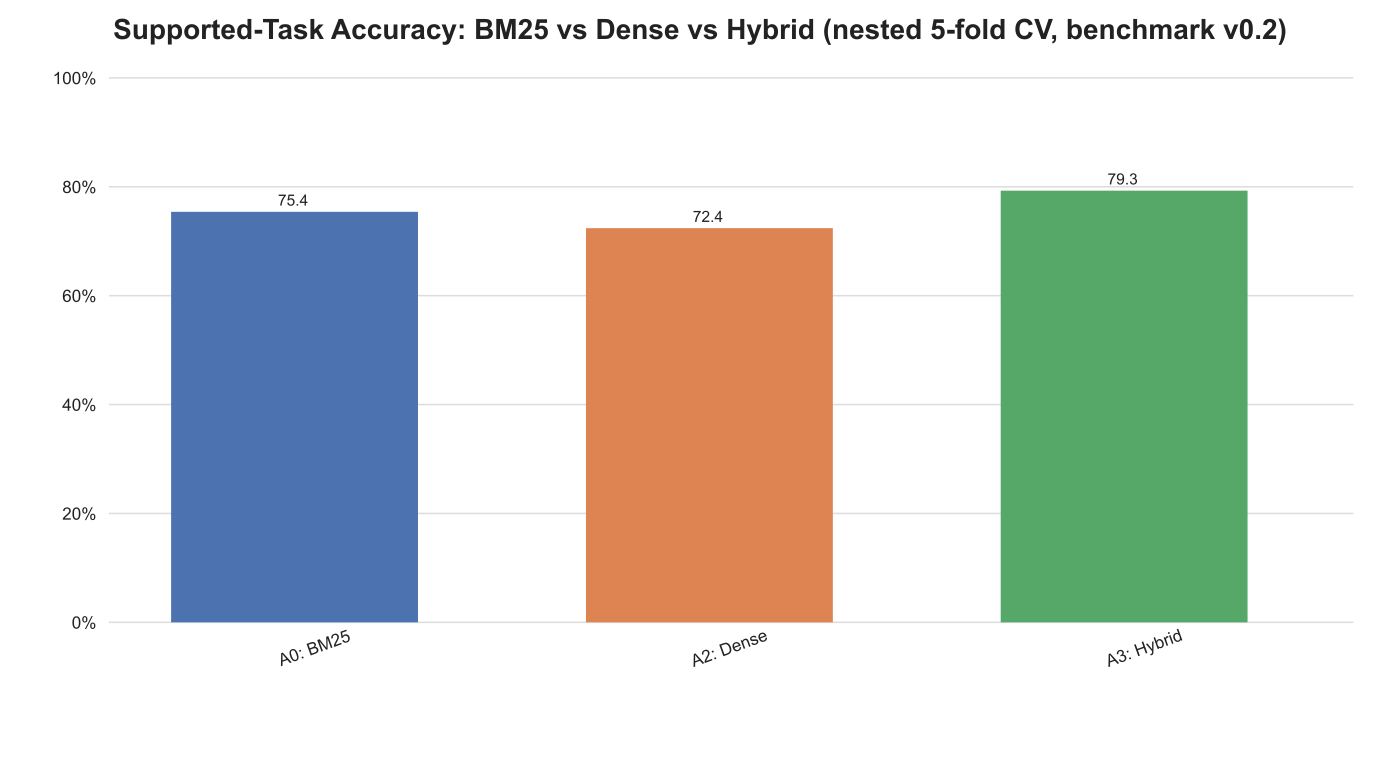
\includegraphics[width=0.48\linewidth]{figures/fig1_baseline_vs_improved_accuracy_v0.2.png}
  \caption{Accuracy on non-OOD queries (pooled; $n=135$ and $159$) for BM25, dense-only, and hybrid
  retrieval under nested 5-fold CV. Left: v0.1. Right: v0.2. The BM25$\to$hybrid gain is similar in size
  on both versions; its exact-test significance differs (Table~\ref{tab:holm}) and rests on a few queries
  (Table~\ref{tab:sens}).}
  \label{fig:accuracy}
\end{figure*}

By query type (v0.1), hybrid retains BM25's 100\% on canonical and safety-sensitive queries while
improving most on low-overlap-paraphrase; single-keyword and OOD queries remain the hardest
categories for both systems, and v0.2 has a similar shape (Figure~\ref{fig:bytype}, Appendix~\ref{app:figs}).

\paragraph{OOD and ambiguity detection.} On v0.1, AUROC is 0.867 for OOD detection (feature: absolute
top-1 score) and 0.784 for ambiguity detection (feature: margin). On v0.2, with 50 instead of 15 OOD
queries, OOD AUROC is 0.901, and the tuned OOD detector raises the rejection rate on OOD queries from the
baseline's 34.0\% to 68.0\% (17/50 to 34/50), which \textbf{survives Holm correction} (Holm-adjusted
$p=0.00006$). On v0.1 the same comparison was not significant even before correction (raw $p=0.25$).
Combined with margin rejection (A5, \S\ref{sec:ablation}), 38 of the 50 OOD queries are rejected.
Ambiguity-detection F1 is 0.310 on v0.1 and 0.496 on v0.2, while AUROC is 0.784 and 0.723.

\paragraph{Calibration.} Isotonic calibration reduces ECE for all four confidence signals we tested, by
46.9--84.1\% (the dense-similarity signal gains least). For the hybrid's own fused-score signal, which
the rest of the paper uses, ECE falls from 0.2741 to 0.0537 on v0.1 (80.4\%; Figure~\ref{fig:reliability},
left) and from 0.3237 to 0.0738 on v0.2 (77.2\%; right). A paired bootstrap test of the reduction gives
one-sided $p\leq0.0001$ on both benchmarks (the resolution of 10,000 resamples), and this is the
\textbf{only comparison in the family that survives Holm correction on both benchmark versions}
(Table~\ref{tab:holm}). Selective answering at 50\% coverage achieves 10.7\% error vs.\ 30.7\% unconditional
on v0.1; risk-coverage curves for both versions are in Figure~\ref{fig:riskcoverage} (Appendix~\ref{app:figs}).

\begin{figure*}[t]
  \centering
  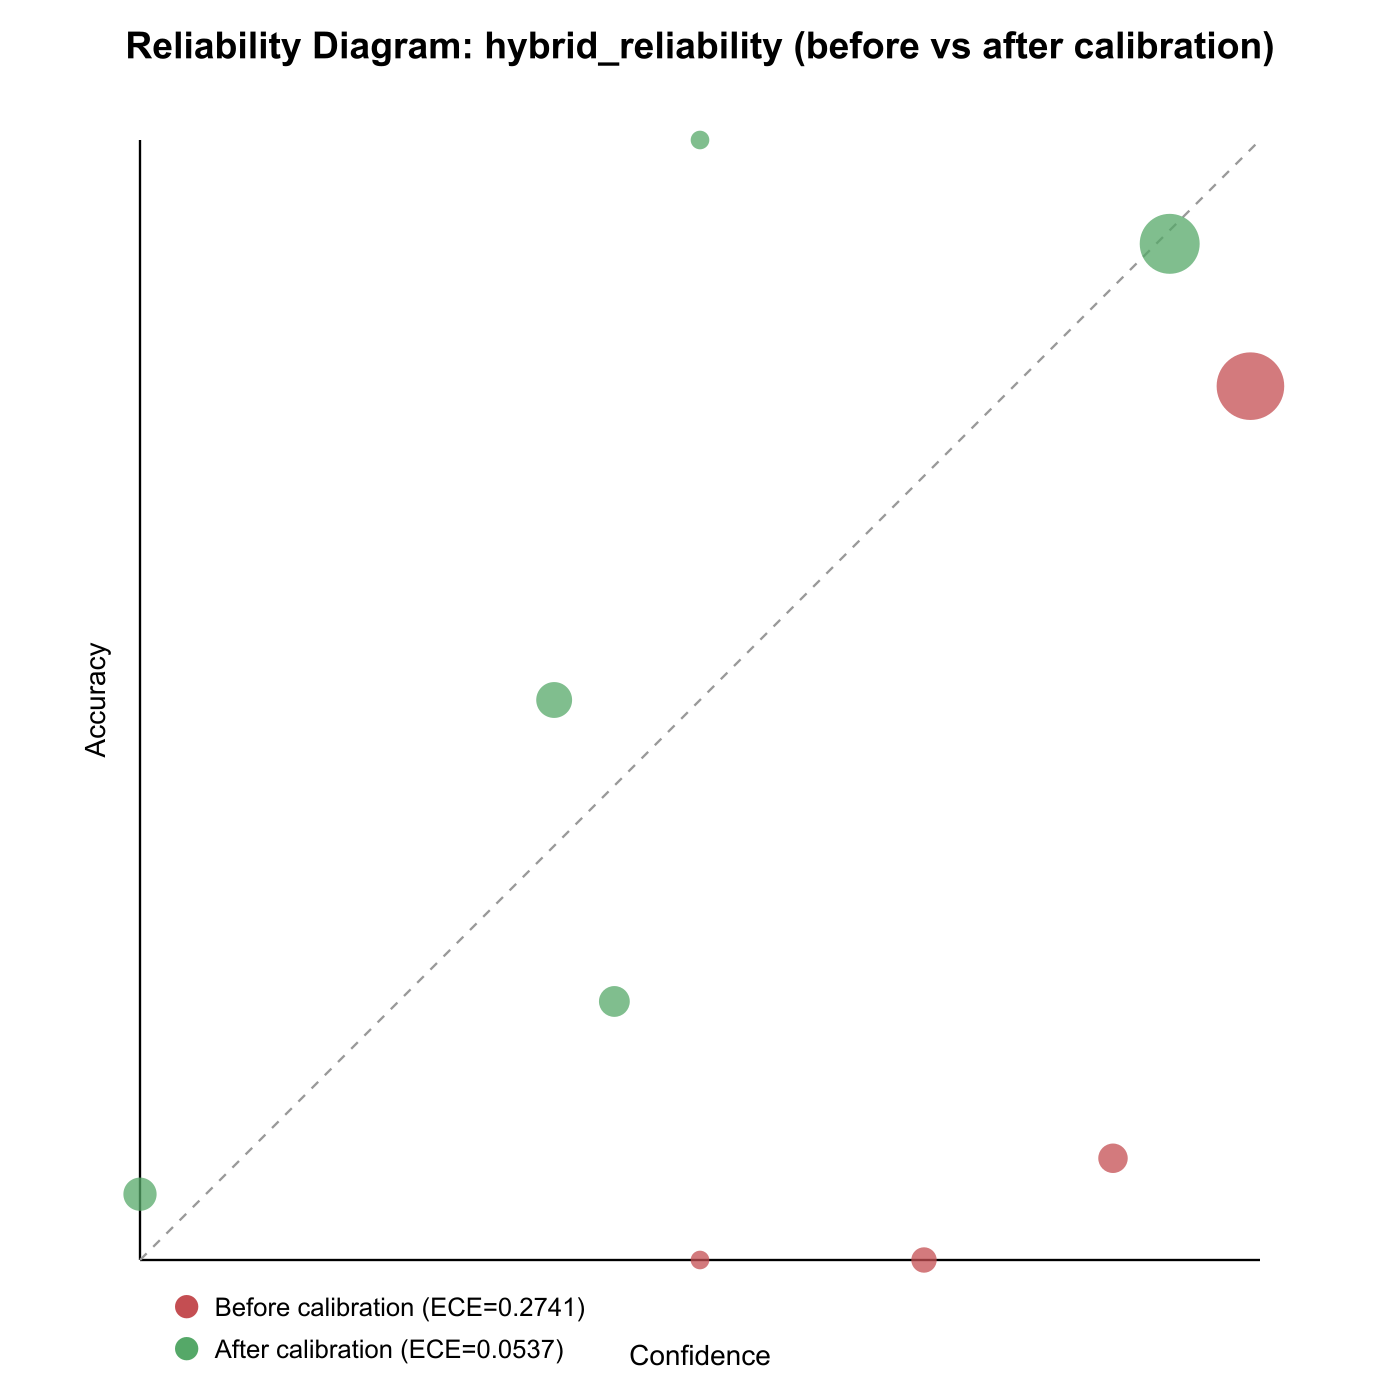
\includegraphics[width=0.40\linewidth]{figures/fig3_reliability_diagram.png} \hspace{0.08\linewidth}
  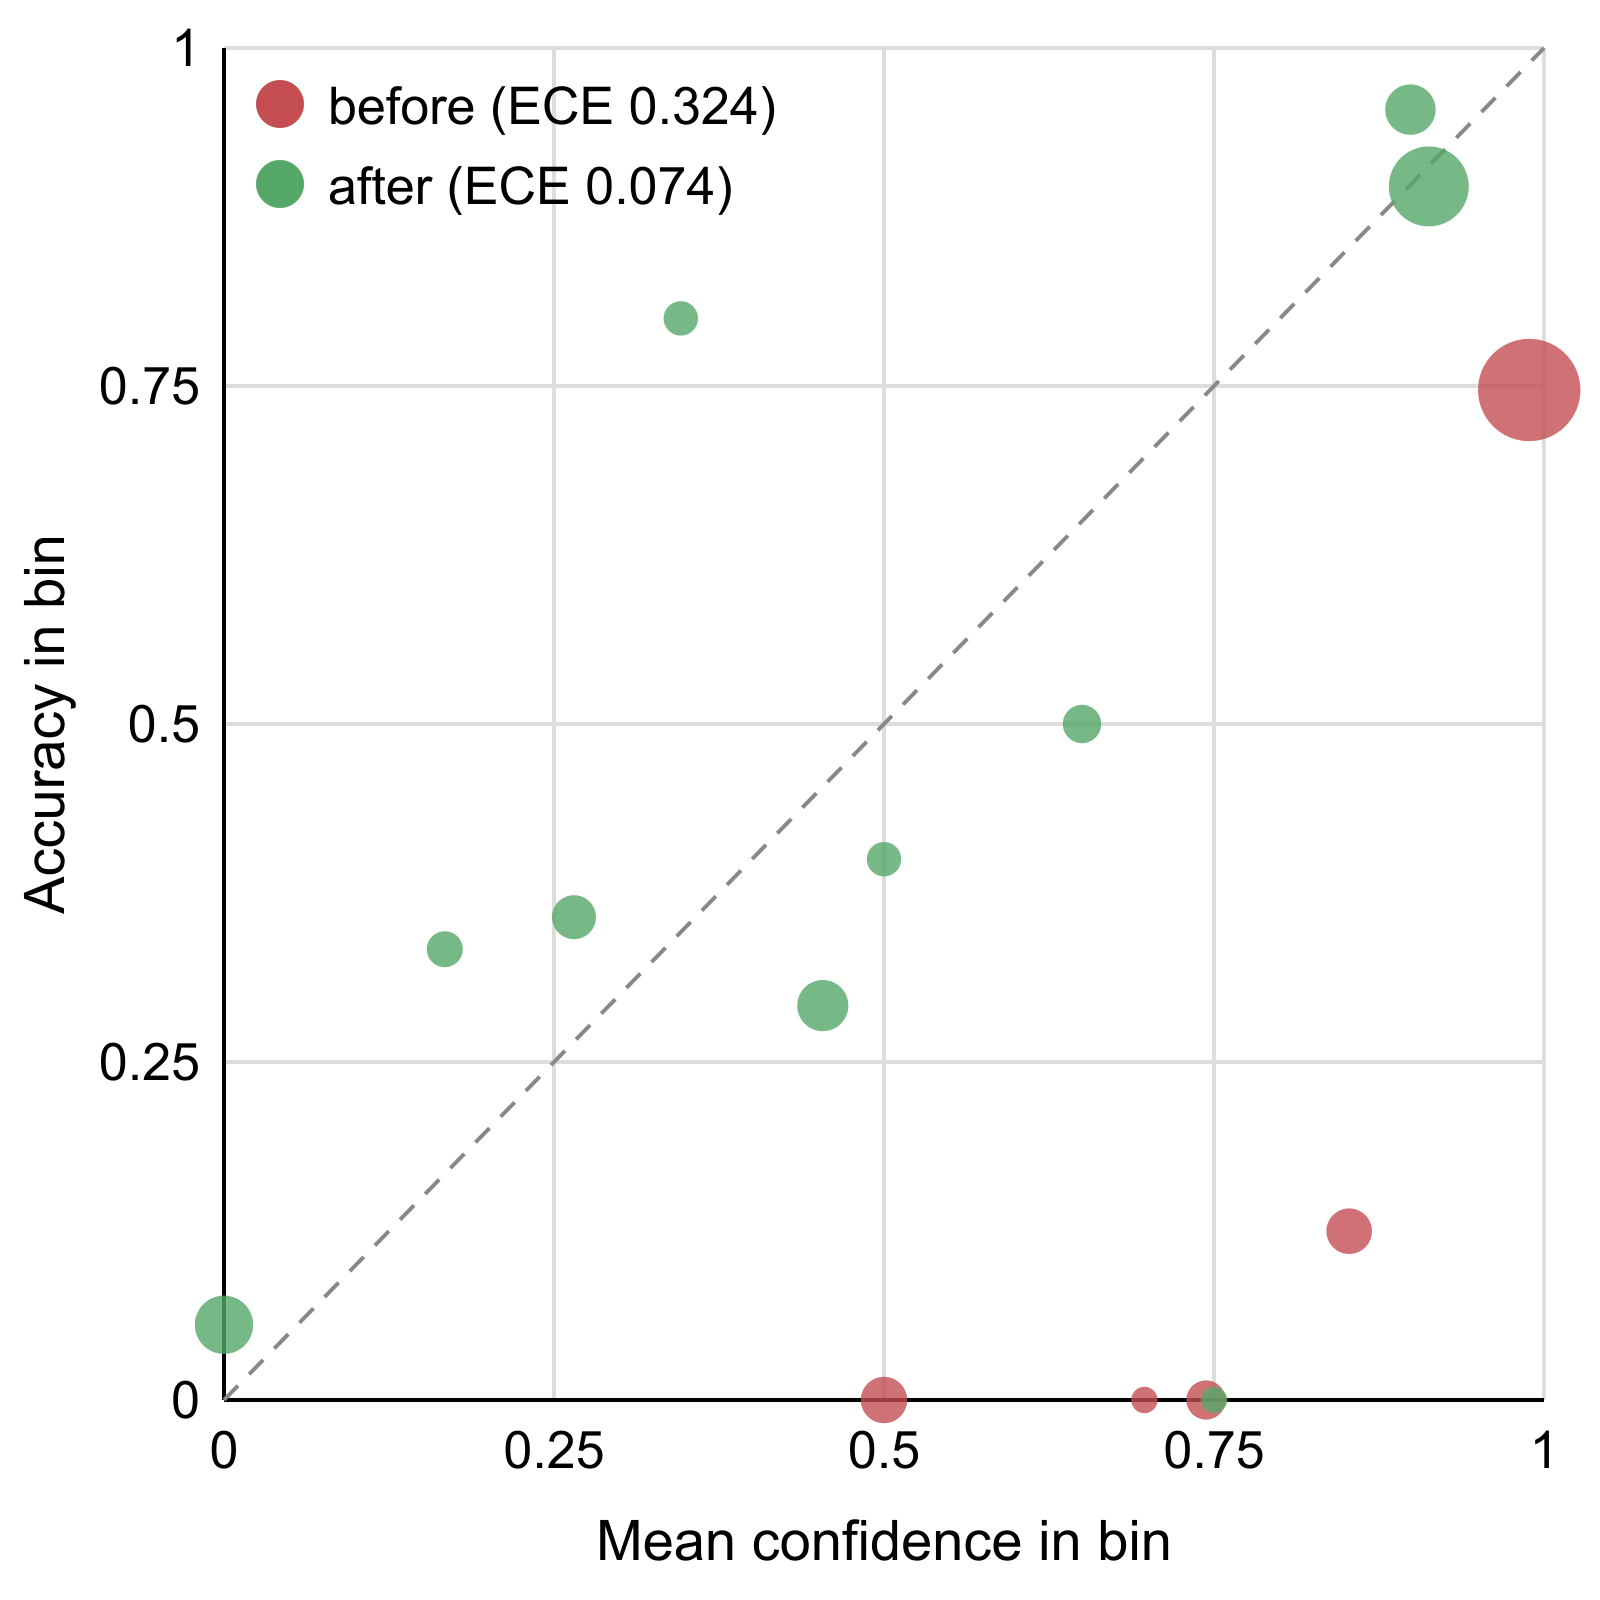
\includegraphics[width=0.40\linewidth]{figures/fig3_reliability_diagram_v0.2.png}
  \caption{Reliability diagram for the hybrid system's fused-score confidence, before vs.\ after isotonic
  calibration (10 equal-width bins; dot area grows with the number of predictions in the bin; dashed line:
  perfect calibration). Left: v0.1. Right: v0.2.}
  \label{fig:reliability}
\end{figure*}

\begin{table}[t]
  \centering
  \small
  \setlength{\tabcolsep}{3pt}
  \begin{tabular}{@{}llrrc@{}}
    \toprule
    \textbf{Ver.} & \textbf{Comparison} & \textbf{Raw $p$} & \textbf{Holm} & \textbf{Sig.} \\
    \midrule
    v0.1 & Acc., hybrid vs. BM25 & 0.0156 & 0.0469 & \textbf{Yes} \\
    v0.1 & Acc., hybrid vs. dense & 0.1460 & 0.2920 & No \\
    v0.1 & OOD rej., tuned vs. base & 0.25 & 0.2920 & No \\
    v0.1 & Calib. ECE reduction & 0.0001 & 0.0004 & \textbf{Yes} \\
    v0.2 & Acc., hybrid vs. BM25 & 0.0703 & 0.0703 & No \\
    v0.2 & Acc., hybrid vs. dense & 0.0127 & 0.0255 & \textbf{Yes} \\
    v0.2 & OOD rej., tuned vs. base & 0.000015 & 0.00006 & \textbf{Yes} \\
    v0.2 & Calib. ECE reduction & 0.0001 & 0.0003 & \textbf{Yes} \\
    \bottomrule
  \end{tabular}
  \caption{Holm-corrected significance ($\alpha=0.05$; exploratory, see \S\ref{sec:methods}); Ver.\ is
  the benchmark version. The calibration $p$ of 0.0001 is the resolution limit of the bootstrap.
  Bootstrap 95\% CIs: accuracy vs.\ BM25 [2.2, 8.9]pp (v0.1) and [0.6, 7.5]pp (v0.2); accuracy vs.\
  dense [$-$0.7, 9.6]pp and [1.9, 11.9]pp; ECE reduction [0.128, 0.283] and [0.172, 0.295].}
  \label{tab:holm}
\end{table}

\paragraph{Sensitivity to bare-keyword queries.} A blind reviewer disagreed with our labels on
several short ambiguous queries (\S\ref{sec:kappa}), so we re-evaluated on subsets that drop them
(Table~\ref{tab:sens}). The rule (an ambiguous-labeled query with a single token, applied to both versions)
was stated before the subset results were computed, but we already knew from the full-benchmark analysis
which query BM25 won, so this analysis is post hoc and exploratory. The fusion weight and detector
thresholds were \emph{not} re-tuned on the reduced sets, while calibration was re-fit. Three results stand
out. (i) The BM25$\to$hybrid gain is stable in size, $+4.9$ to $+5.8$ points on every reduced subset, each
with 7--0 discordant queries in hybrid's favor. (ii) The hybrid-over-dense advantage on v0.2 is not stable:
it falls to raw $p=0.057$ without the new bare-keyword queries and to $p=0.227$ on answerable queries only.
(iii) The calibration gain is unchanged (77--84\% relative ECE reduction across all rows, one-sided bootstrap
$p\leq0.0001$ in each). OOD rejection is not recomputed: relabeling ambiguous queries cannot change it,
because ambiguous and answerable queries are both non-OOD negatives and the OOD queries are identical in
every subset. Finally, on answerable queries only, v0.1 and v0.2 are the same 121 queries, so v0.2 adds no
answerable evidence.

\begin{table*}[t]
  \centering
  \small
  % AUTO-GENERATED by research/experiments/generate_sensitivity_table.js -- do not edit by hand.
\begin{tabular}{@{}llrccr@{}}
    \toprule
    \textbf{Ver.} & \textbf{Evaluated on} & \textbf{n} & \textbf{BM25$\to$Hyb.} & \textbf{Dense$\to$Hyb.} & \textbf{ECE red.} \\
    \midrule
    v0.1 & all queries & 135 & +5.2 (0.016) & +4.4 (0.146) & 80\% \\
    v0.1 & w/o 9 bare-keyword & 126 & +5.6 (0.016) & +4.8 (0.146) & 80\% \\
    v0.2 & all queries & 159 & +3.8 (0.070) & +6.9 (0.013) & 77\% \\
    v0.2 & w/o 17 new bare-keyword & 142 & +4.9 (0.016) & +5.6 (0.057) & 81\% \\
    v0.2 & w/o all 26 bare-keyword & 133 & +5.3 (0.016) & +6.0 (0.057) & 84\% \\
    v0.1/v0.2 & answerable only & 121 & +5.8 (0.016) & +4.1 (0.227) & 78/81\% \\
    \bottomrule
  \end{tabular}

  \caption{Sensitivity to bare-keyword ambiguous queries (post hoc). Cells show the hybrid's accuracy
  gain in points over BM25 and over dense retrieval, with the exact McNemar $p$ (unadjusted) in
  parentheses; ECE red.\ is the relative ECE reduction from isotonic calibration re-fit on the
  subset; $n$ counts non-OOD queries evaluated. Fusion weight and thresholds were not re-tuned.}
  \label{tab:sens}
\end{table*}

\paragraph{Intent-held-out generalization (Split B).} GroupKFold over 171 derived intent groups
(v0.2; 0 groups split across folds, verified programmatically) shows that hybrid accuracy and OOD
detection do not depend on intent overlap between tuning and test: the hybrid answers exactly the same
number of non-OOD queries correctly under both splits (126/159 on v0.2 and 104/135 on v0.1), and OOD AUROC
is 0.898 vs.\ 0.901 on v0.2. Calibration, while still a large improvement, is measurably
\textbf{attenuated on held-out intents}: a 69.0\% vs.\ 77.2\% relative ECE reduction on v0.2 and 76.4\%
vs.\ 80.4\% on v0.1 (Table~\ref{tab:splitb}). The v0.1 detection numbers are noisier, consistent with its
small OOD subset.

\begin{table}[t]
  \centering
  \small
  \setlength{\tabcolsep}{3pt}
  \begin{tabular}{@{}llrrr@{}}
    \toprule
    \textbf{Ver.} & \textbf{Metric} & \textbf{Split A} & \textbf{Split B} & \textbf{$\Delta$} \\
    \midrule
    v0.1 & Non-OOD acc. & 104/135 & 104/135 & 0 \\
    v0.1 & OOD AUROC & 0.867 & 0.849 & $-$0.018 \\
    v0.1 & Ambig. F1 & 0.310 & 0.300 & $-$0.010 \\
    v0.1 & Calib. ECE & .274$\to$.054 & .274$\to$.065 & $+$0.011 \\
    v0.2 & Non-OOD acc. & 126/159 & 126/159 & 0 \\
    v0.2 & OOD AUROC & 0.901 & 0.898 & $-$0.003 \\
    v0.2 & Ambig. F1 & 0.496 & 0.479 & $-$0.017 \\
    v0.2 & Calib. ECE & .324$\to$.074 & .324$\to$.101 & $+$0.027 \\
    \bottomrule
  \end{tabular}
  \caption{Split A (class-stratified) vs.\ Split B (intent-held-out). For ECE, $\Delta$ is the change in
  post-calibration ECE (higher is worse).}
  \label{tab:splitb}
\end{table}

\section{Ablation, Functional, and Safety Evaluation}
\label{sec:ablation}

\paragraph{Ablation (v0.1 / v0.2).} A0 (BM25) = 71.9\%/75.5\%; A1 (BM25, no substring bonus) is
\textbf{identical} to A0 on both benchmarks (0 command differences on 150 or 209 queries) --- the bonus
fires on 47/150 v0.1 queries but never changes the top-1 winner, a null result we report plainly rather
than let the bonus's presence imply an untested effect. A2 (dense) = 72.6\%/72.3\%; A3 (hybrid, nested-CV)
= 77.0\%/79.2\%. The following are selective accuracies on the answered queries, averaged over folds. A4
(+margin rejection) reaches 88.5\% at 70.8\% coverage on v0.1; A5 (+OOD detection) reaches 90.1\% at
69.5\% coverage (10/15 OOD rejected). On v0.2, A5 is \emph{lower} at \emph{lower} coverage (82.2\% at
58.9\%; 38/50 OOD rejected); we did not analyze why beyond noting that v0.2 adds only OOD and ambiguous
queries. A6 (+calibration) makes the same decisions as A5 but its confidence has ECE 0.054 instead of
0.274 on v0.1 (Figure~\ref{fig:ablation}, Appendix~\ref{app:figs}).

\paragraph{Functional evaluation.} Sandboxed execution (disposable temp directories, never the host
machine) on a deliberately narrow, explicitly-scoped 15/150-query subset (git + filesystem,
placeholder-free, non-interactive, host-safe gold commands only). Gold commands: 100\% functional
success (validates benchmark quality). Retrieved (hybrid) commands: 93.3\% functional success, zero
cases of textually-correct-but-functionally-broken --- a positive result that covers only 10\% of
the benchmark by design.

\paragraph{Safety evaluation.} A deterministic, rule-based classifier with four risk levels (low,
medium, high, critical), written from general domain knowledge before inspecting per-query outcomes,
was evaluated against the benchmark's pre-existing risk labels: 89.6\% exact four-level accuracy (112/125
gold commands), 95\%/95\% precision/recall on the actionable risky-vs.-not-risky decision, and no
dangerous-direction misses (no critical- or high-risk command was ever tagged safe). On retrieved commands,
accuracy holds (90.0\%) but risky-binary precision drops to 0.826 --- a retrieval-error artifact, not a
classifier defect. On v0.2, exact accuracy and recall shift modestly downward (83.9\%/0.864) because the
classifier --- deliberately not re-tuned against new examples --- was authored before v0.2's new gold
commands existed, surfacing the same documented gaps, not new ones.

\section{Blind Re-Annotation of a Sample of AI-Authored Queries}
\label{sec:kappa}

v0.2's 59 new queries were authored and adjudicated by an AI agent under human direction. To check for
systematic labeling error, we drew a stratified, seed-42 sample of 14 of them (8 OOD-labeled, 6
ambiguous-labeled) and had one reviewer judge each query fresh, blind to its original label, as clearly
answerable, ambiguous, or OOD. The reviewer is the project's human director, who directed the original
authoring at a summary level but had not seen these 14 labels; the check is therefore blind but only
partially independent. The reviewer was also shown only the query text, not the command list, whereas our
labels are defined relative to that list (a query is ambiguous if the list holds several distinct commands
that match it), so part of any disagreement may reflect different definitions rather than labeling error.
Cohen's $\kappa=0.6316$, below our pre-specified 0.7 target. Agreement was perfect on the 8 OOD-labeled
items (8/8), and all three disagreements were among the 6 ambiguous-labeled ones: ``ffmpeg'' and ``pip''
(single-token tool names) and ``list running processes'' (a short category phrase), each of which we had
labeled ambiguous but the reviewer judged to have one obvious default command. The other three ambiguous
items (``copy a file'', ``security'', ``system'') were confirmed. With $n=14$ the estimate is coarse: a
post hoc bootstrap 95\% interval for $\kappa$ is [0.39, 1.00], and one flipped item would move it
materially. All sampled OOD labels, on which the OOD-rejection result rests, were confirmed; the ambiguous
labels are the uncertain ones, which is why \S\ref{sec:results} reports how the conclusions change when
ambiguous queries are excluded. The disputed items are not all single-token, so the ``answerable only''
rows of Table~\ref{tab:sens}, which drop every ambiguous query, are the ones free of this label
uncertainty.

\section{Discussion}

The clearest result concerns reliability, not accuracy. Post-hoc isotonic calibration removes most of the
baseline's overconfidence (80\% and 77\% relative ECE reduction for the hybrid's confidence on v0.1 and
v0.2). It is the only compared effect that is significant after correction on both benchmark versions, it
survives intent-held-out evaluation with some attenuation (69--76\% vs.\ 77--80\%), and it is unchanged when
bare-keyword or all ambiguous queries are removed (Table~\ref{tab:sens}). OOD rejection is the second solid
result, but only once the OOD subset grew from 15 to 50 queries, and all 8 of its labels that we
re-annotated were confirmed. The accuracy gain over BM25 is real in size but not established in
significance: it is similar on both versions ($+5.2$ and $+3.8$ points), and every discordant query but one
favors the hybrid, yet the exact test has only 7--8 discordant queries to work with, so a single query
(``system'') moves it across the threshold. The hybrid-over-dense result on v0.2 depends on three new
bare-keyword queries. We draw two lessons. First, at this benchmark size, significance statements about
accuracy differences are fragile to individual queries, the power concern raised by
\citet{card2020littlepower}; effect sizes with intervals are more informative than $p$-values here. Second,
v0.2's additional queries are all OOD or ambiguous, so they test detection and calibration but add no
answerable evidence: expanding the benchmark helped the OOD question and did not help the accuracy question.
Ambiguity detection remains weak, and our re-annotation suggests part of the difficulty is that the
ambiguous label itself is unsettled for short queries.

\section{Conclusion and Future Work}
\label{sec:conclusion}

A lightweight, fully offline, non-LLM hybrid retriever with post-hoc isotonic calibration substantially
improves the reliability of a shipped BM25 command-retrieval baseline. The most defensible results are the
calibration improvement, which holds on both benchmark versions, on held-out intents, and when ambiguous
queries are removed, and the OOD-rejection improvement, which is significant on the larger OOD subset.
The hybrid's accuracy gain over BM25 is consistent in size but statistically fragile, the hybrid-over-dense
advantage on v0.2 depends on a few bare-keyword queries, and ambiguity detection is weak. All significance
analyses are exploratory. Future work, in priority order: (1) a two-annotator re-annotation of all 59
AI-authored queries, for which a written codebook (defining labels relative to the command list) and a
pre-declared analysis protocol are ready, followed by adjudication and a corrected, frozen benchmark
version; (2) a confirmatory analysis specified before running on that benchmark; (3) more answerable
queries, since v0.2 adds none; (4) an independent human-labeled safety set not derived from the
classifier's own logic; (5) expanding the corpus toward the planned 500--800 human-validated intents, and
functional evaluation beyond 15 tasks; and (6) a human-preference study. Items (1)--(5) need human effort
and cannot responsibly be replaced by bulk automated generation.

% Invisible marker: build.sh reads its page number to check the 8-page limit. Per the ACL formatting
% guidelines, the Limitations and Ethical Considerations sections below come after the conclusion and do
% not count toward the page limit, so the marker sits at the end of the conclusion. Keep it here.
\label{endofbody}

\section*{Limitations}

\begin{itemize}
  \item \textbf{Benchmarks are not independent, and v0.2 adds no answerable evidence.} v0.2 contains
  all of v0.1; the 121 answerable queries are identical in both versions, and every difference comes
  from added OOD and ambiguous queries. Results on the two versions are not independent replications,
  and their Holm families are not independent either.
  \item \textbf{Fragile accuracy inference.} The exact tests on accuracy rest on 7--8 discordant
  queries; one query decides whether BM25$\to$hybrid is significant on v0.2, and three decide
  hybrid-vs.-dense (\S\ref{sec:results}). We treat the accuracy gain as suggestive.
  \item \textbf{Exploratory statistics.} The Holm family and the choice of calibration as the primary
  hypothesis were fixed after the raw results were known, and the sensitivity analysis is post hoc
  (fusion weight and thresholds were not re-tuned on the reduced sets). No result here is confirmatory.
  \item \textbf{Label uncertainty in AI-authored queries.} v0.2's 59 new queries were authored and
  adjudicated by an AI agent under human direction. A blind re-annotation of 14 by one partially
  independent reviewer, who did not see the command list, gave $\kappa=0.63$ (\S\ref{sec:kappa}): OOD
  labels were confirmed, ambiguous labels were not (3/6 disagreed). The two-annotator protocol has not
  been run, and v0.1's own ambiguous labels have not been re-annotated at all.
  \item \textbf{Ambiguity detection is weak} (F1 0.31--0.50 under both class-stratified and
  intent-held-out evaluation), and the ambiguous label itself is unsettled for short queries.
  \item \textbf{Canonical-query independence.} All 25 canonical queries are verbatim-equal to a corpus
  intent, so 100\% canonical accuracy is a positive-control sanity check, not evidence of language
  understanding; the paraphrase, low-overlap, polysemy, and ambiguous types carry the capability claims.
  \item \textbf{Ground-truth defects.} Three benchmark items have gold or acceptable commands outside the
  searched corpus (\S\ref{sec:system}). They do not change comparisons between systems, but they should be
  corrected in a later version.
  \item \textbf{Corpus scale, platform, and vetting.} 279 Windows-visible intents (431 raw records), small
  relative to generation-oriented corpora and single-platform; records were checked by script, not
  validated one by one; the planned 500--800-intent expansion is not done.
  \item \textbf{Calibration under intent shift.} The ECE reduction attenuates on intent-held-out
  evaluation (80\% to 76\% on v0.1, 77\% to 69\% on v0.2), and isotonic calibration is sensitive to small
  samples.
  \item \textbf{Evaluation scope.} No human-preference study; a fixed embedding model; no end-to-end
  latency measurement of the hybrid; functional evaluation covers only 15 of 150 queries and treats success
  as exit code 0, not verified side effects; the safety classifier is evaluated against the benchmark's own
  risk labels.
  \item \textbf{Literature coverage.} Our literature search was limited, so we make no claim of priority
  or novelty beyond the comparisons cited.
\end{itemize}

\section*{Ethical Considerations}

TermAssist retrieves from a fixed, curated command library rather than generating arbitrary shell commands,
which bounds its possible outputs to commands in that library. The library was checked by script rather than
reviewed command by command (\S\ref{sec:system}), so this bound is weaker than full human vetting, and a
retrieved command can still be inappropriate for a given user's intent; our own baseline audit found the
deployed system is frequently \emph{confidently} wrong. We evaluate command risk with a separate,
deterministic safety classifier (\S\ref{sec:ablation}) specifically because retrieval correctness and command
risk are orthogonal concerns: a correctly retrieved command can still be destructive if misapplied, and no
component in this study executes a retrieved command against a user's real system. All functional-evaluation
command execution in this study ran in disposable, sandboxed temporary directories, never against a host
machine. We disclose the AI-assisted authorship of part of our benchmark (\S\ref{sec:system}) and the
below-target result of our own partially independent re-annotation of it (\S\ref{sec:kappa}) rather than omit
or minimize either.

\bibliography{references}

\appendix

\section{Additional Figures}
\label{app:figs}

\begin{figure*}[t]
  \centering
  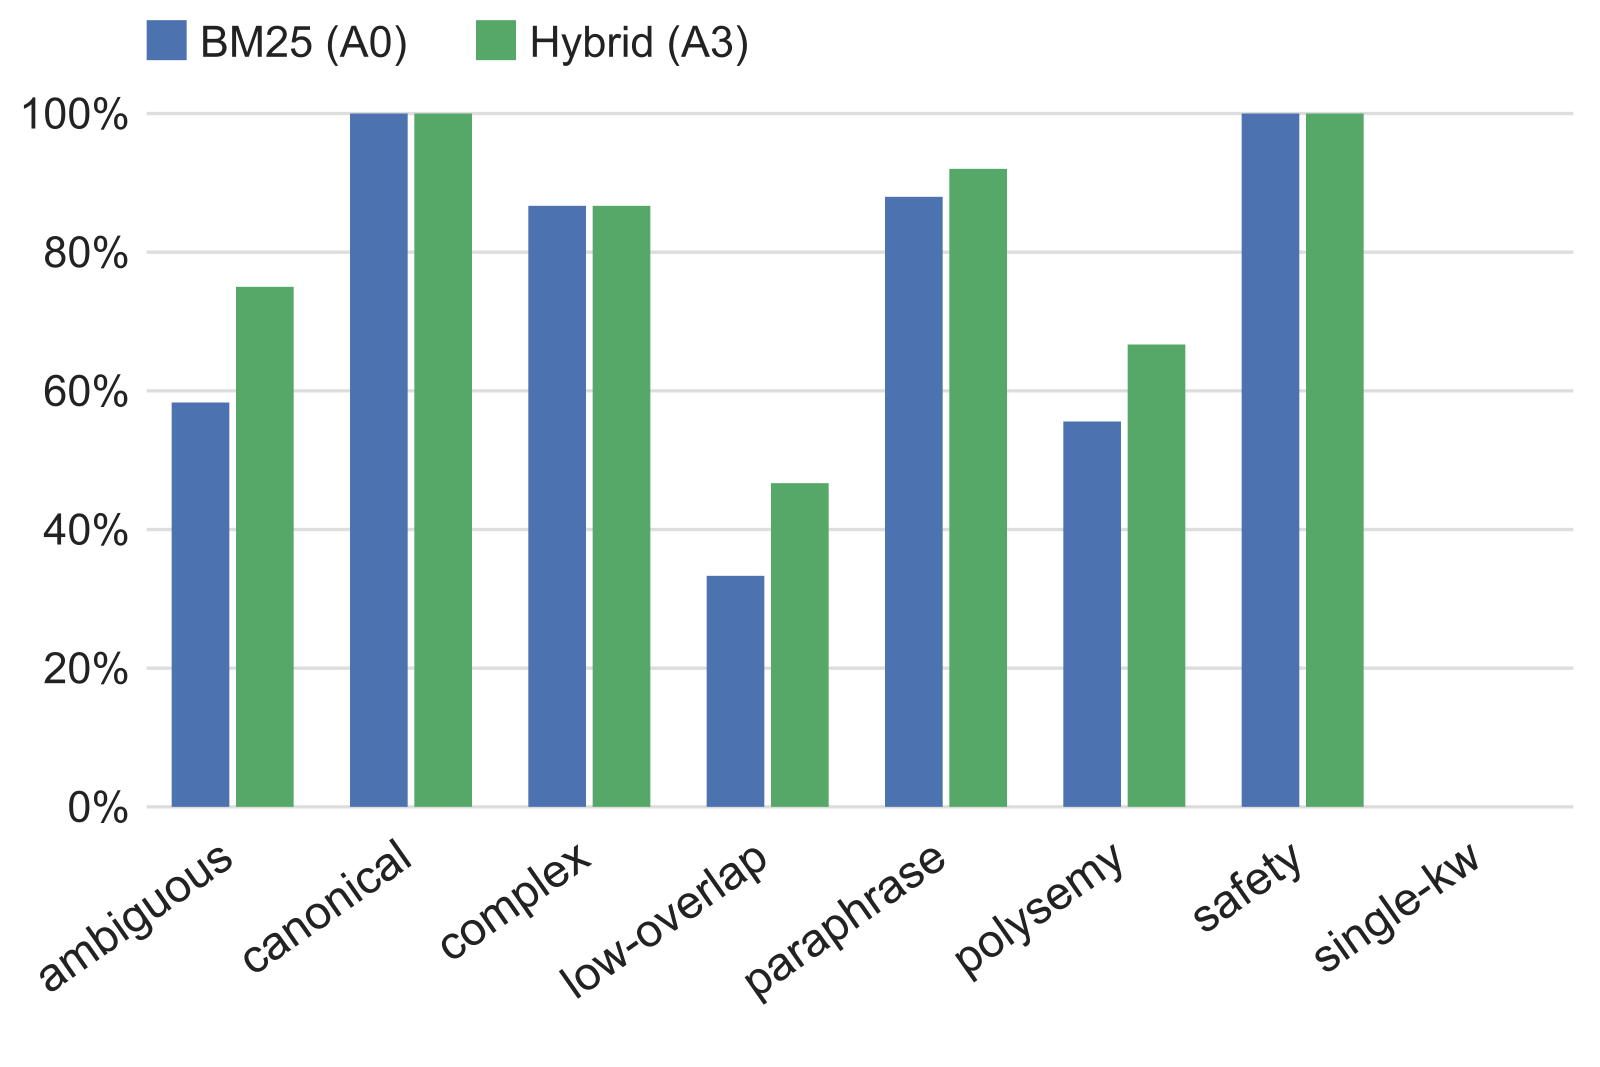
\includegraphics[width=0.48\linewidth]{figures/fig2_accuracy_by_query_type.png} \hfill
  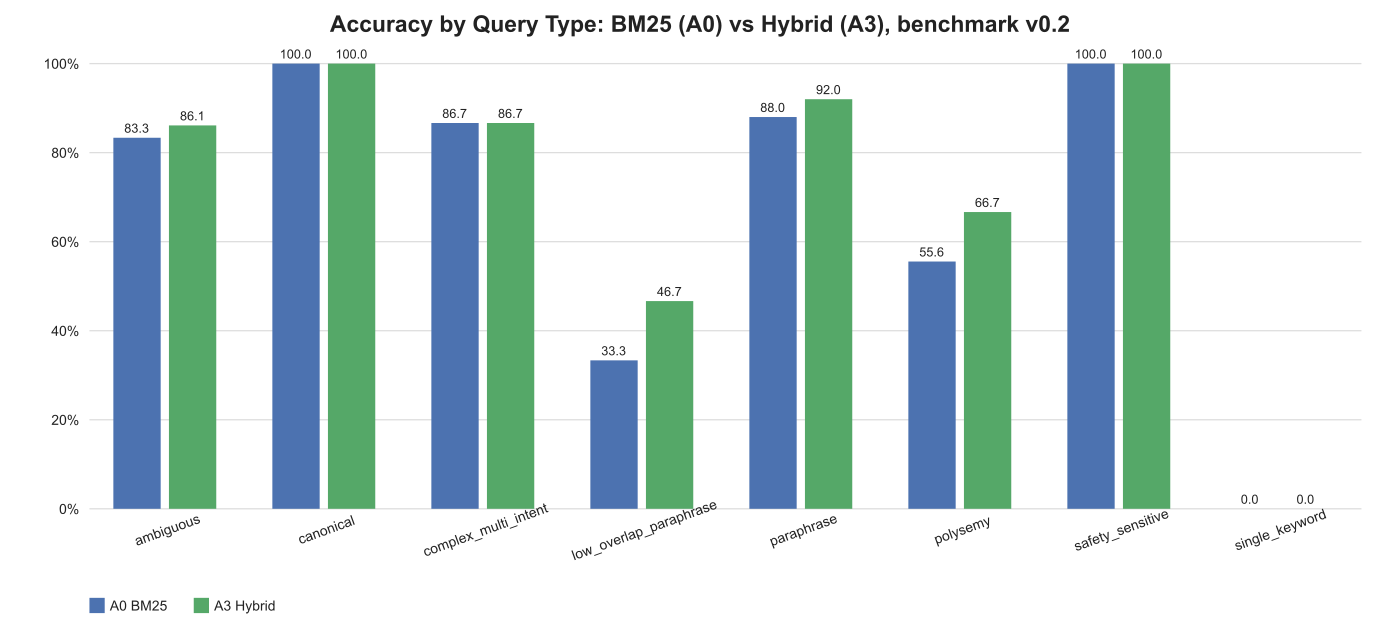
\includegraphics[width=0.48\linewidth]{figures/fig2_accuracy_by_query_type_v0.2.png}
  \caption{Accuracy by query type, BM25 (A0) vs.\ hybrid (A3). Single-keyword queries are 0\% for both
  systems, so their bars are empty. Left: v0.1. Right: v0.2.}
  \label{fig:bytype}
\end{figure*}

\begin{figure*}[t]
  \centering
  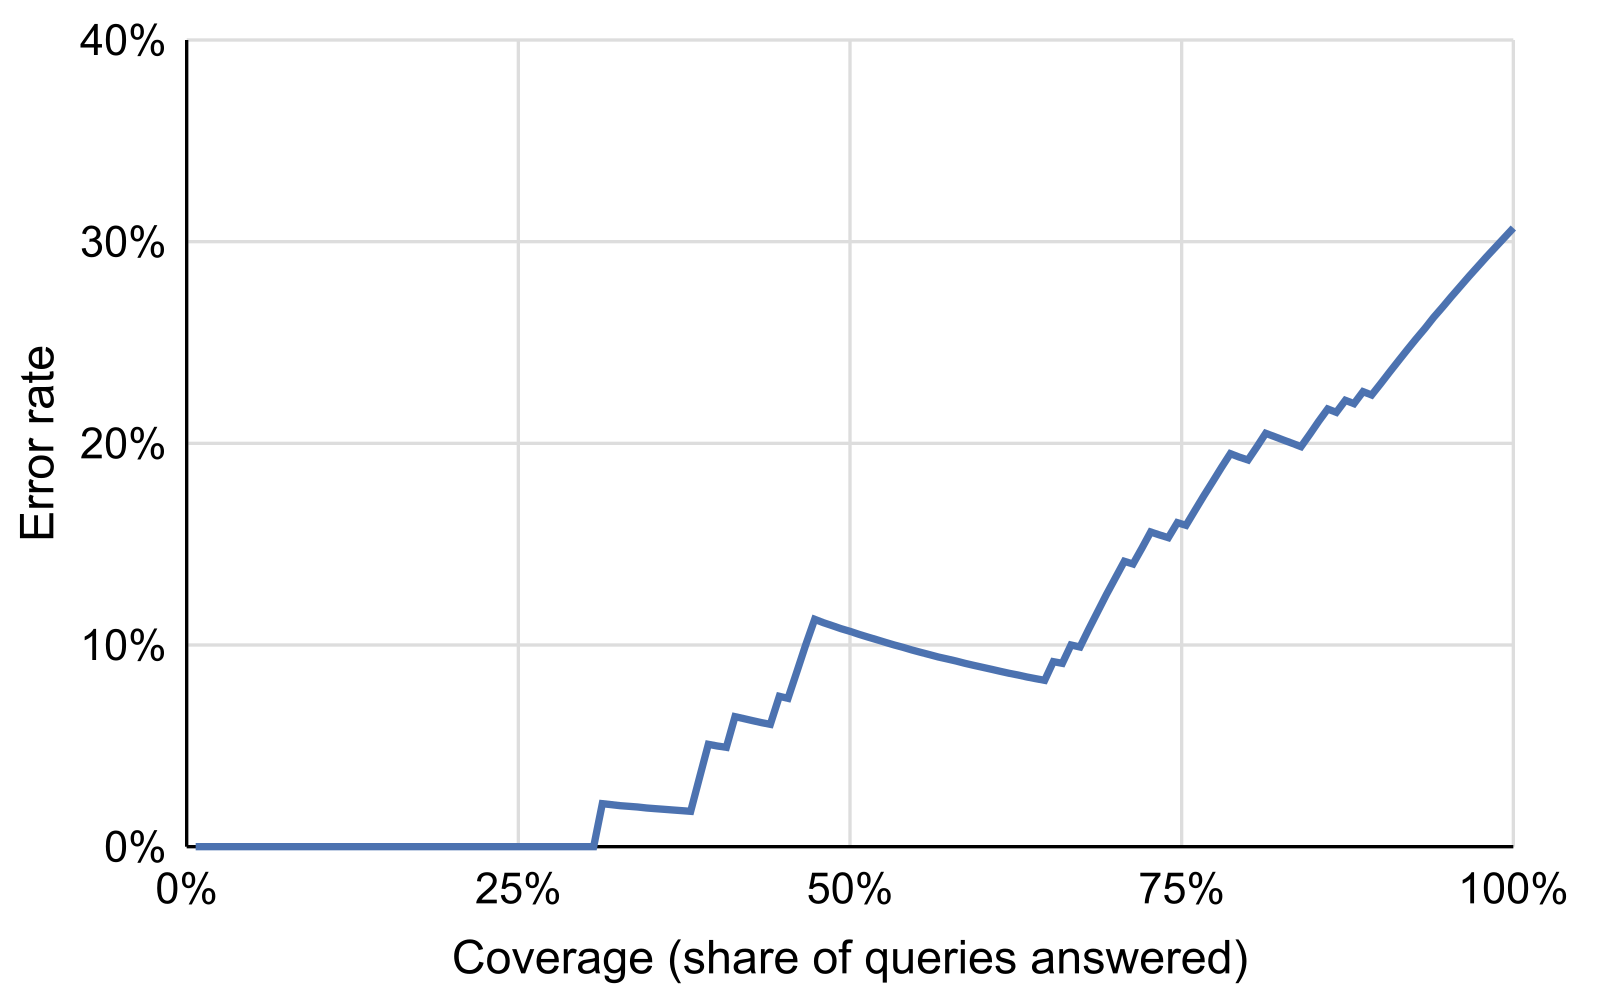
\includegraphics[width=0.48\linewidth]{figures/fig4_risk_coverage_curve.png} \hfill
  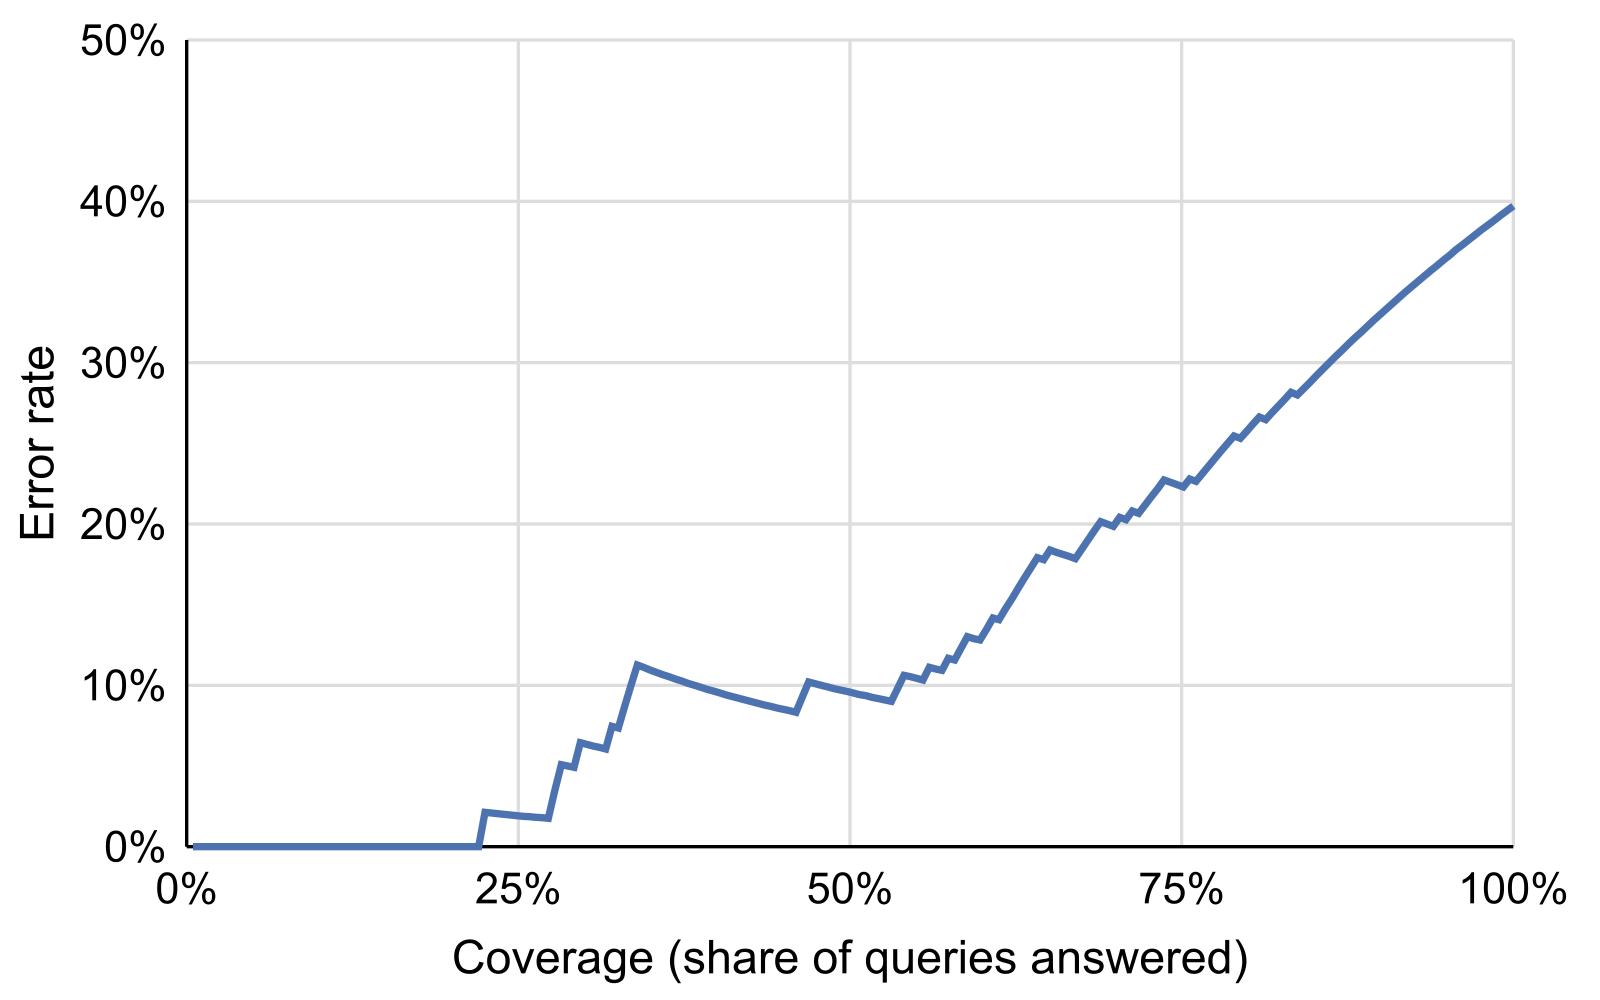
\includegraphics[width=0.48\linewidth]{figures/fig4_risk_coverage_curve_v0.2.png}
  \caption{Risk-coverage curve for the hybrid system: queries are answered in order of decreasing
  confidence, and the error rate is computed over the answered share. Left: v0.1. Right: v0.2.}
  \label{fig:riskcoverage}
\end{figure*}

\begin{figure*}[t]
  \centering
  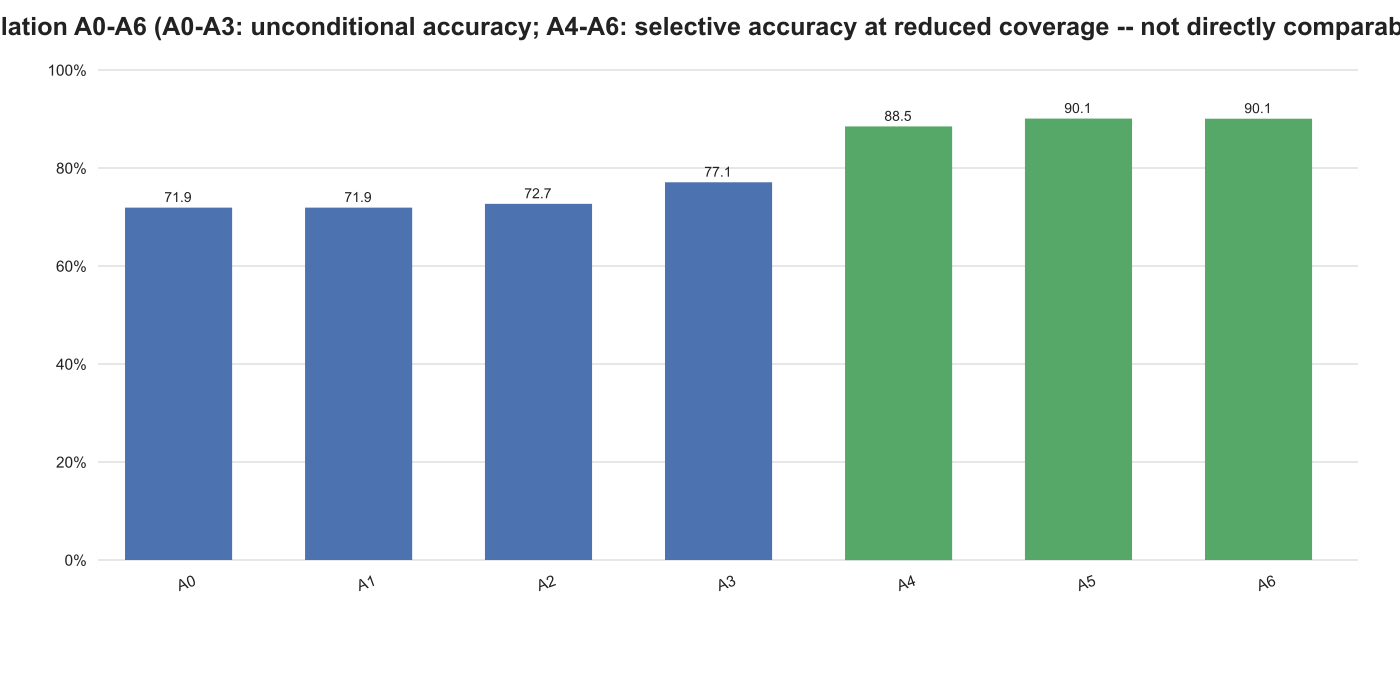
\includegraphics[width=0.48\linewidth]{figures/fig5_ablation_A0_A6.png} \hfill
  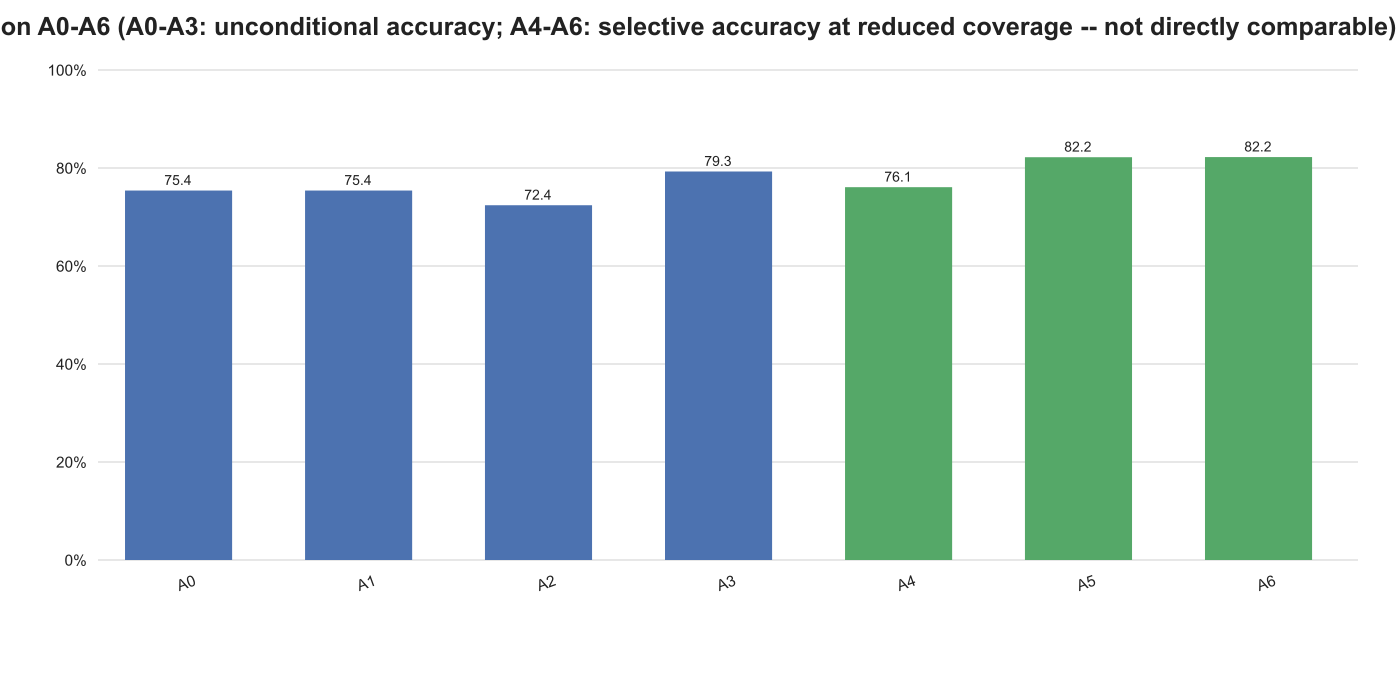
\includegraphics[width=0.48\linewidth]{figures/fig5_ablation_A0_A6_v0.2.png}
  \caption{Ablation A0--A6. A0--A3: accuracy on all non-OOD queries (pooled). A4--A6: selective accuracy on
  the queries each configuration answers (mean over folds), at reduced coverage, so not directly comparable
  to A0--A3. Left: v0.1. Right: v0.2.}
  \label{fig:ablation}
\end{figure*}


\end{document}

% ============================================================================
% NOTE (not part of the paper -- delete before submitting)
% ============================================================================
% This is the FINAL/CAMERA-READY build: real author info, no anonymization.
% Most ACL/EACL-family venues want an ANONYMIZED PDF for the actual
% review-stage submission and only reveal author info at camera-ready time
% after acceptance -- confirm which stage you're at before sending this PDF
% anywhere. Use main_review.tex for the review-stage submission instead.
%
% Page count: 9 pages total as of the last build (7 pages body text, under
% the ACL/EACL SRW 8-page limit; References on pages 8-9, which don't count
% against that limit). Recheck after any edit to content.tex, figures, or
% tables -- don't assume it still fits.
